\documentclass[11pt,a4paper]{article}

\usepackage[T1]{fontenc}
\usepackage[utf8]{inputenc}
\usepackage{lmodern}
\usepackage[margin=2.4cm]{geometry}
\usepackage{graphicx}
\usepackage{amsmath}
\usepackage{booktabs}
\usepackage{caption}
\usepackage{microtype}
\usepackage[section]{placeins}
\renewcommand{\topfraction}{0.85}\renewcommand{\textfraction}{0.1}\renewcommand{\floatpagefraction}{0.75}
\usepackage{xcolor}
\usepackage[colorlinks=true,linkcolor=blue!50!black,urlcolor=blue!50!black,citecolor=blue!50!black]{hyperref}

\graphicspath{{figures/}}
\captionsetup{font=small,labelfont=bf}
\setlength{\parskip}{0.5em}
\setlength{\parindent}{0pt}

\title{Multi-label Diagnosis of 14 Thoracic Diseases from Chest X-rays\\
\large Four architectures compared, explanations measured against radiologists' boxes,\\ calibrated probabilities and a containerised demo}
\author{Hayder Methneni \and Khaled Ayedi}
\date{Deep Learning Avanc\'e --- TEK-UP, ING-5, 2026--2027\\ (also submitted for Big Data)}

\begin{document}
\maketitle

\begin{abstract}
We detect 14 thoracic diseases, each independently, from frontal chest X-rays of the NIH ChestX-ray14 dataset, using a patient-wise split to avoid leakage. Our first model, a DenseNet121 trained with a class-weighted loss, reaches a mean AUC of 0.799 on the official test set of 25{,}596 images. We then repeated our ablation study on four architectures (DenseNet121, ResNet50, EfficientNet-B0, ConvNeXt-Tiny; 16 training runs) and evaluated every run on the test set with patient-level bootstrap confidence intervals and paired tests. Three findings hold across architectures:
\begin{itemize}
  \item fine-tuning the backbone is essential;
  \item class weighting does not improve AUC (worse on three of four architectures, a gap four times the seed-to-seed noise) and is the cause of the over-confident scores;
  \item the same subgroups are harder for every architecture (patients under 40 and bedside AP films), while there is no gap between men and women.
\end{itemize}
ConvNeXt-Tiny is the best single model (\textbf{test AUC 0.809}), and an ensemble of the four reaches \textbf{0.816} [0.810, 0.821]. With plain cross-entropy and temperature scaling the outputs are calibrated probabilities (test ECE below 0.013). We also measured Grad-CAM against 984 bounding boxes drawn by radiologists: ConvNeXt-Tiny's heatmap peak falls inside the box 44\% of the time, against 22\% for a point always at the image centre, while two architectures barely beat that baseline. The four models are served side by side through ONNX Runtime, FastAPI and React, packaged with Docker Compose and checked by continuous integration. This is a research and educational demo, not a diagnostic tool.
\end{abstract}

\begin{center}
\fbox{\begin{minipage}{0.93\textwidth}
\textbf{What changed since the first review.}
\begin{itemize}\setlength{\itemsep}{1pt}
  \item \emph{``Why not train other models and run the same study on them?''} We did: four architectures $\times$ three variants, plus repeated seeds (Section~\ref{sec:benchmark}).
  \item Every model is now evaluated on the test set with confidence intervals and paired significance tests, instead of single validation numbers.
  \item The over-confidence of the first model is explained (weighted loss) and fixed; the app now shows calibrated probabilities (Section~\ref{sec:calibration_bench}).
  \item Grad-CAM is no longer only illustrated but measured against expert bounding boxes (Section~\ref{sec:localisation}), and per-subgroup performance is reported.
  \item The app serves the four models and their ensemble, with a side-by-side comparison view.
  \item \emph{``What is the role of Docker?''} Answered in Section~\ref{sec:docker}: it delivers the trained models as a reproducible, two-container service, which we ran end to end.
\end{itemize}
\end{minipage}}
\end{center}

\section{Introduction}
Chest radiography is one of the most common imaging exams, and reading it is slow and subject to variability between readers. Automatic multi-label classification of findings is a standard benchmark for medical image analysis with deep learning. The task is difficult for three reasons: findings are visually subtle, several can co-occur in one image, and the labels are noisy.

Our goals were to (i) build a sound, reproducible training and evaluation pipeline, (ii) report honest numbers on the official test split, (iii) make the predictions inspectable with Grad-CAM, and (iv) deliver the model as a working application rather than a notebook. After the first review we added (v) a comparison of four architectures under one protocol, with statistical tests, calibration, and a measurement of the explanations against expert annotations. The full code, tests and instructions are in the project repository (\url{https://github.com/khldd/chest-xray-diagnosis}).

\section{Dataset}
We use the NIH ChestX-ray14 dataset~\cite{wang2017chestxray}: 112{,}120 frontal X-rays from 30{,}805 patients, each labelled with any of 14 findings (or ``No Finding''). The labels were extracted automatically from radiology reports, so they contain noise that no model can overcome. The images (about 45 GB) are not stored in the repository.

\paragraph{Splits.} We keep the official split: \texttt{train\_val\_list} (86{,}524 images) and \texttt{test\_list} (25{,}596 images), the latter used only for the final evaluation. From the training pool we hold out 15\% as validation using \texttt{GroupShuffleSplit} grouped by patient identifier (seed 42), so that no patient appears in both training and validation. This gives 73{,}916 training, 12{,}608 validation and 25{,}596 test images. A unit test checks that the patient sets are disjoint.

\paragraph{Labels and imbalance.} Each image gets a 14-dimensional multi-hot vector; ``No Finding'' is the all-zero vector. The classes are strongly imbalanced (Table~\ref{tab:classes}): Infiltration is present in 16.0\% of training images, while Hernia is present in only 0.15\% (113 images).

\begin{table}[htbp]
\centering
\begin{tabular}{lrrrr}
\toprule
Disease & Train positives & Prevalence (\%) & \texttt{pos\_weight} & Test AUC \\
\midrule
Atelectasis & 7{,}003 & 9.47 & 9.6 & 0.751 \\
Cardiomegaly & 1{,}453 & 1.97 & 49.9 & 0.871 \\
Consolidation & 2{,}482 & 3.36 & 28.8 & 0.729 \\
Edema & 1{,}201 & 1.62 & 60.5 & 0.840 \\
Effusion & 7{,}415 & 10.03 & 9.0 & 0.816 \\
Emphysema & 1{,}274 & 1.72 & 57.0 & 0.909 \\
Fibrosis & 1{,}051 & 1.42 & 69.3 & 0.809 \\
Hernia & 113 & 0.15 & 653.1 & 0.933 \\
Infiltration & 11{,}853 & 16.04 & 5.2 & 0.693 \\
Mass & 3{,}452 & 4.67 & 20.4 & 0.792 \\
Nodule & 4{,}042 & 5.47 & 17.3 & 0.738 \\
Pleural Thickening & 1{,}870 & 2.53 & 38.5 & 0.766 \\
Pneumonia & 742 & 1.00 & 98.6 & 0.688 \\
Pneumothorax & 2{,}287 & 3.09 & 31.3 & 0.849 \\
\bottomrule
\end{tabular}

\caption{Per-class training prevalence, loss weight and test AUC. The loss weight is the ratio of negatives to positives in the training split.}
\label{tab:classes}
\end{table}

\section{Method}
\paragraph{Preprocessing.} Images are resized to $224\times224$, replicated to three channels, and normalised with ImageNet statistics. The only training augmentation in the main model is a random horizontal flip; evaluation uses no augmentation.

\paragraph{Model.} We use DenseNet121~\cite{huang2017densenet} pretrained on ImageNet and replace the 1000-way classifier with a linear layer from 1024 features to 14 outputs. All 6.97 million parameters are fine-tuned. Each output is passed through a sigmoid at inference time, giving an independent probability per disease.

\paragraph{Loss.} Training uses binary cross-entropy with logits and a per-class positive weight $w_c = N^{-}_c / N^{+}_c$ computed on the training split (Table~\ref{tab:classes}), which ranges from 5.2 for Infiltration to 653 for Hernia. The motivation is that a model can reach a low loss by predicting ``absent'' for rare findings; Section~\ref{sec:ablations} tests whether this weighting actually helps.

\paragraph{Optimisation.} Adam with learning rate $10^{-4}$, batch size 32, up to 15 epochs on a Kaggle T4 GPU. After every epoch the mean validation AUC is computed and the checkpoint with the best value is kept. The final pipeline writes the full training state (weights, optimiser, epoch, history) so a run can be resumed, and logs to MLflow.

\paragraph{Metric.} Because the data are imbalanced and multi-label, we report the area under the ROC curve (AUC) per class and its mean over the 14 classes. Accuracy would be misleading here.

\paragraph{Explanations.} Grad-CAM~\cite{selvaraju2017gradcam} is computed on the last feature layer (\texttt{features.norm5}) for a chosen disease. It produces a coarse heatmap of the regions that increased that disease's score.

\section{Results}
\subsection{Main model}
The selected checkpoint reaches a mean AUC of \textbf{0.831} on the validation split and \textbf{0.7987} on the official test split. Table~\ref{tab:classes} lists the per-class test AUCs and Figure~\ref{fig:auc} plots them. Hernia (0.933), Emphysema (0.909) and Cardiomegaly (0.871) are the best-detected findings; Pneumonia (0.688) and Infiltration (0.693) are the weakest.

\begin{figure}[htbp]
\centering
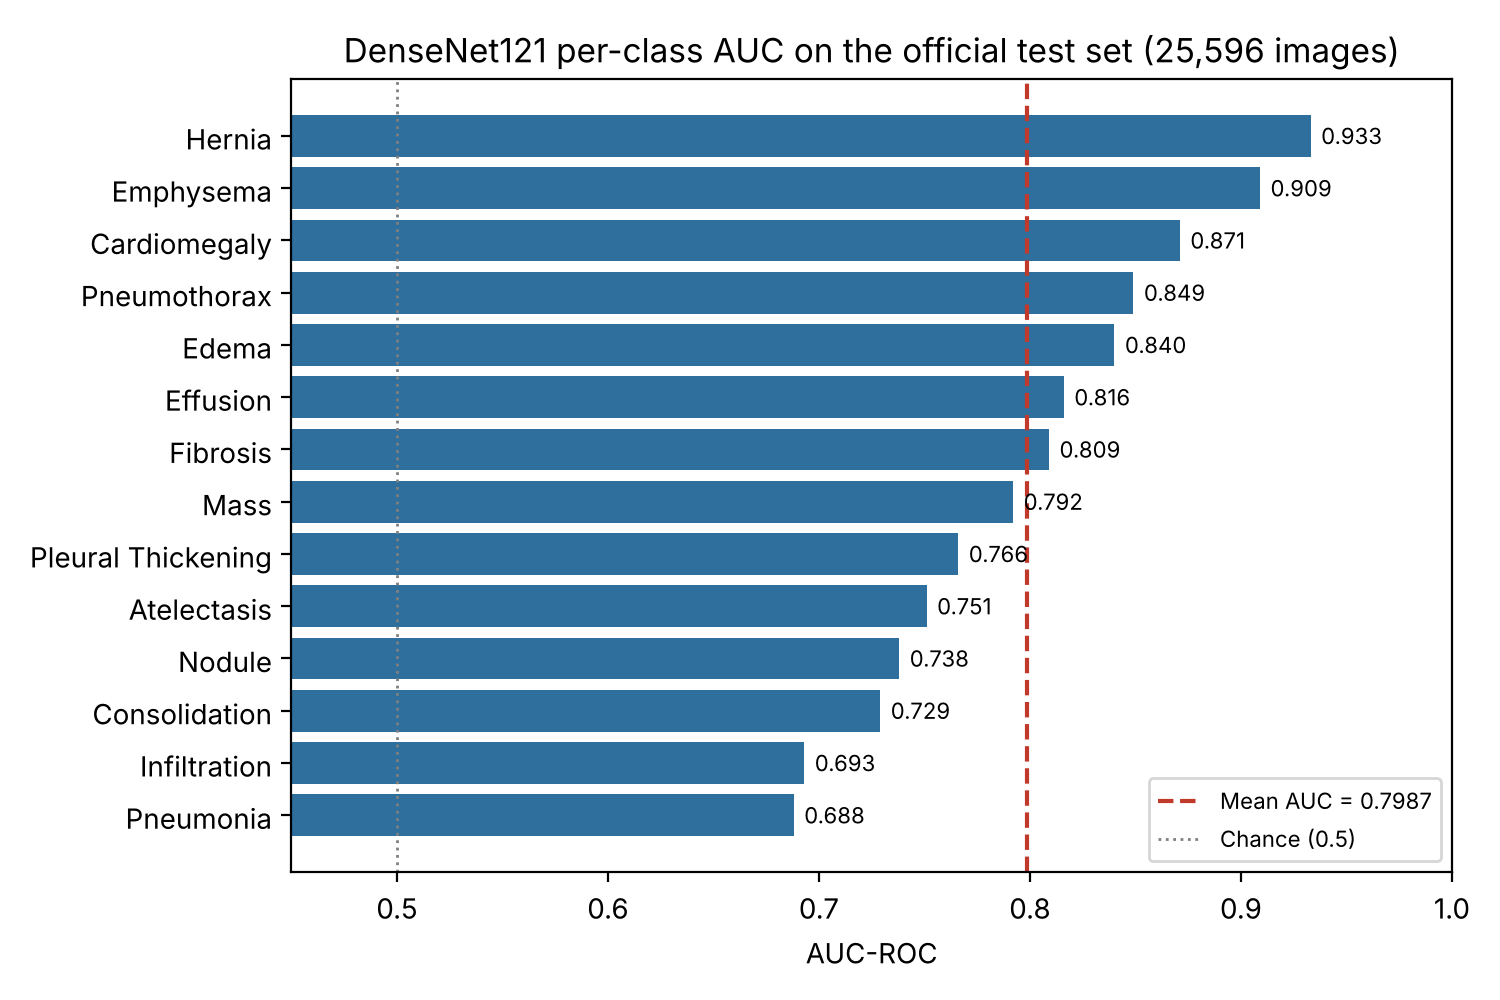
\includegraphics[width=0.82\textwidth]{test_auc_per_class.png}
\caption{Per-class AUC of the final model on the official test set (25{,}596 images).}
\label{fig:auc}
\end{figure}

The gap between validation and test is expected and we do not hide it. The best epoch was selected on the validation set, which makes that number slightly optimistic, and the test patients are different. The weakest classes include findings that are typically diffuse or ambiguous on a frontal film (Infiltration, Pneumonia, Consolidation). Hernia has the highest AUC despite having only 113 training positives; because it is the rarest class, its estimate is likely the least stable, and we did not compute confidence intervals.

\subsection{Threshold metrics and calibration}
\label{sec:calibration}
AUC does not say how the model behaves as a yes/no detector. We therefore choose one cutoff per class on the validation set (maximising sensitivity plus specificity) and apply it unchanged to the test set (Table~\ref{tab:metrics}, Figure~\ref{fig:confusion}). At these cutoffs the mean sensitivity is 0.82 but the mean specificity is 0.62 and the mean precision only 0.14: the model ranks cases well but, because most findings are rare, it produces many false alarms. Average precision (mean 0.27) is far below the AUC (0.80) for the same reason; Pneumonia (AP 0.05) and Fibrosis (AP 0.09) are the extreme cases.

\begin{table}[htbp]
\centering\small
\begin{tabular}{lrrrrrrr}
\toprule
Disease & AUC & AP & Thr. & Sens. & Spec. & PPV & F1 \\
\midrule
Atelectasis & 0.751 & 0.317 & 0.40 & 0.809 & 0.542 & 0.206 & 0.329 \\
Cardiomegaly & 0.871 & 0.307 & 0.23 & 0.851 & 0.712 & 0.114 & 0.201 \\
Consolidation & 0.729 & 0.147 & 0.45 & 0.877 & 0.445 & 0.108 & 0.192 \\
Edema & 0.840 & 0.156 & 0.41 & 0.885 & 0.623 & 0.081 & 0.148 \\
Effusion & 0.816 & 0.495 & 0.42 & 0.883 & 0.560 & 0.309 & 0.458 \\
Emphysema & 0.909 & 0.405 & 0.54 & 0.863 & 0.804 & 0.164 & 0.276 \\
Fibrosis & 0.809 & 0.092 & 0.51 & 0.687 & 0.787 & 0.053 & 0.098 \\
Hernia & 0.933 & 0.468 & 0.03 & 0.895 & 0.829 & 0.017 & 0.034 \\
Infiltration & 0.693 & 0.388 & 0.42 & 0.853 & 0.357 & 0.294 & 0.437 \\
Mass & 0.792 & 0.268 & 0.48 & 0.753 & 0.674 & 0.145 & 0.243 \\
Nodule & 0.738 & 0.207 & 0.47 & 0.713 & 0.639 & 0.118 & 0.203 \\
Pleural Thickening & 0.766 & 0.132 & 0.47 & 0.786 & 0.613 & 0.087 & 0.156 \\
Pneumonia & 0.688 & 0.046 & 0.37 & 0.780 & 0.469 & 0.032 & 0.061 \\
Pneumothorax & 0.849 & 0.384 & 0.50 & 0.869 & 0.657 & 0.228 & 0.361 \\
\midrule
Mean & 0.799 & 0.272 & -- & 0.822 & 0.622 & 0.140 & 0.228 \\
\bottomrule
\end{tabular}

\caption{Test-set metrics per class at the validation-chosen cutoff. AUC and AP (average precision) do not depend on the cutoff.}
\label{tab:metrics}
\end{table}

\begin{figure}[htbp]
\centering
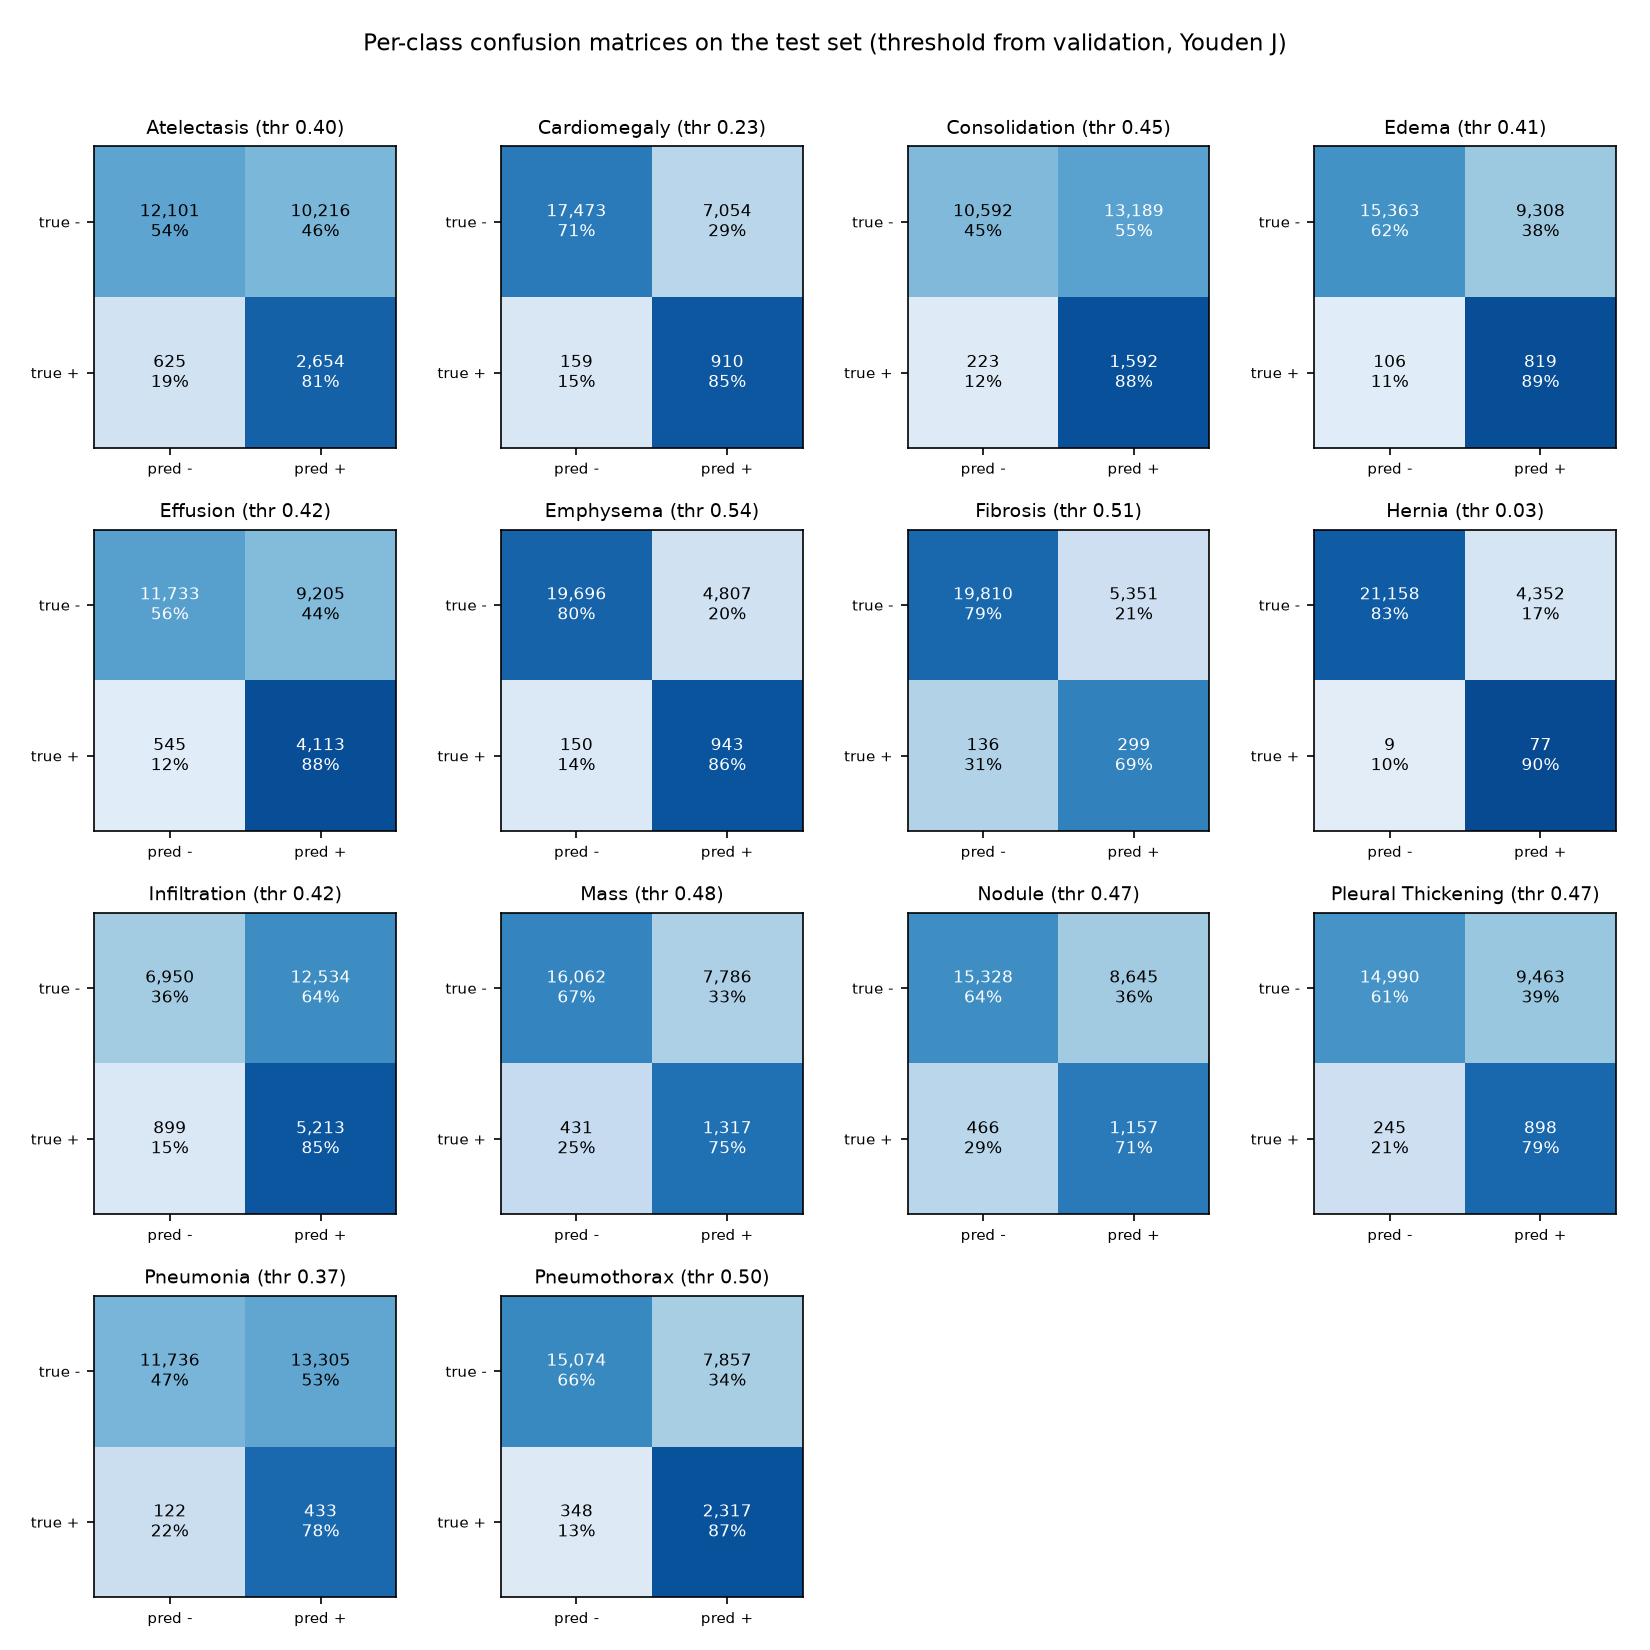
\includegraphics[width=0.95\textwidth]{confusion_matrices.png}
\caption{Per-class confusion matrices on the test set (cell values are counts and row percentages).}
\label{fig:confusion}
\end{figure}

\begin{figure}[htbp]
\centering
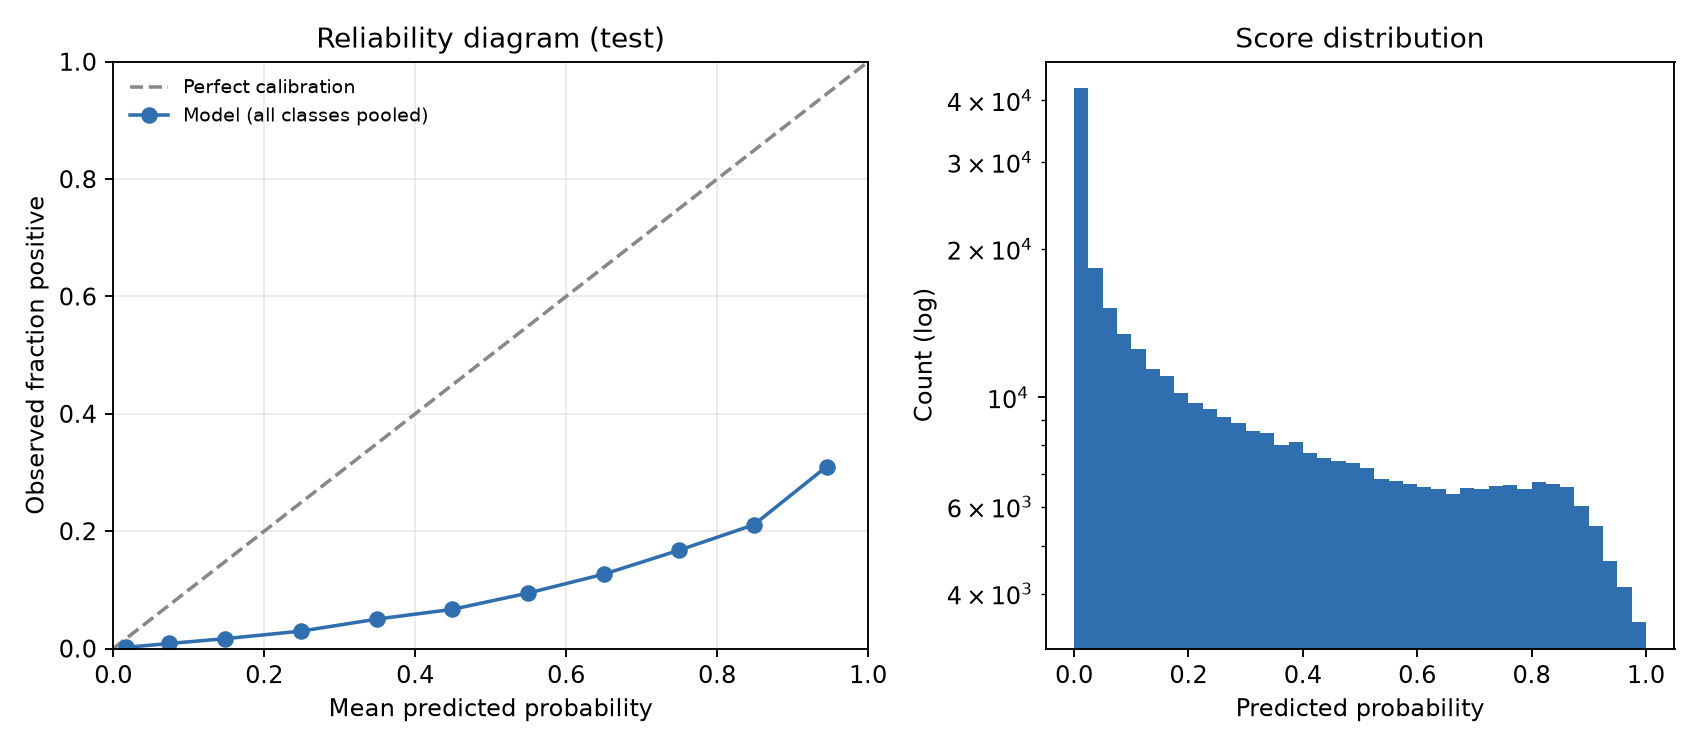
\includegraphics[width=0.88\textwidth]{calibration.png}
\caption{Reliability diagram and score distribution on the test set. Scores are far above the observed frequency: the mean predicted score is 0.38 while 7.6\% of labels are positive.}
\label{fig:calibration}
\end{figure}

The scores of this first model are strongly over-confident (Figure~\ref{fig:calibration}): its sigmoid outputs should be read as rankings, not as probabilities. Section~\ref{sec:calibration_bench} confirms that the weighted loss is the cause, on four architectures, and shows how the models now served are calibrated.

\subsection{Ablations}
\label{sec:ablations}
\IfFileExists{tables/ablations.tex}{%
  To measure what each design choice contributes, we compare variants of the main setup under an identical budget (same data split, optimiser and number of epochs). Table~\ref{tab:ablations} and Figure~\ref{fig:ablation_curves} report the validation mean AUC; the test set is not used for these comparisons.

  \begin{table}[htbp]
  \centering
  \begin{tabular}{llllrr}
\toprule
Run & Backbone & Loss & Augmentation & Best epoch & Val.\ mean AUC \\
\midrule
base\_5ep & fine-tuned & weighted\_bce & flip & 4/5 & 0.8231 \\
baseline\_frozen & frozen & weighted\_bce & flip & 5/5 & 0.7338 \\
unweighted\_bce & fine-tuned & bce & flip & 4/5 & 0.8360 \\
\bottomrule
\end{tabular}

  \caption{Ablation runs. ``Best epoch'' is the epoch with the highest validation mean AUC.}
  \label{tab:ablations}
  \end{table}

  \begin{figure}[htbp]
  \centering
  \IfFileExists{figures/ablation_curves.png}{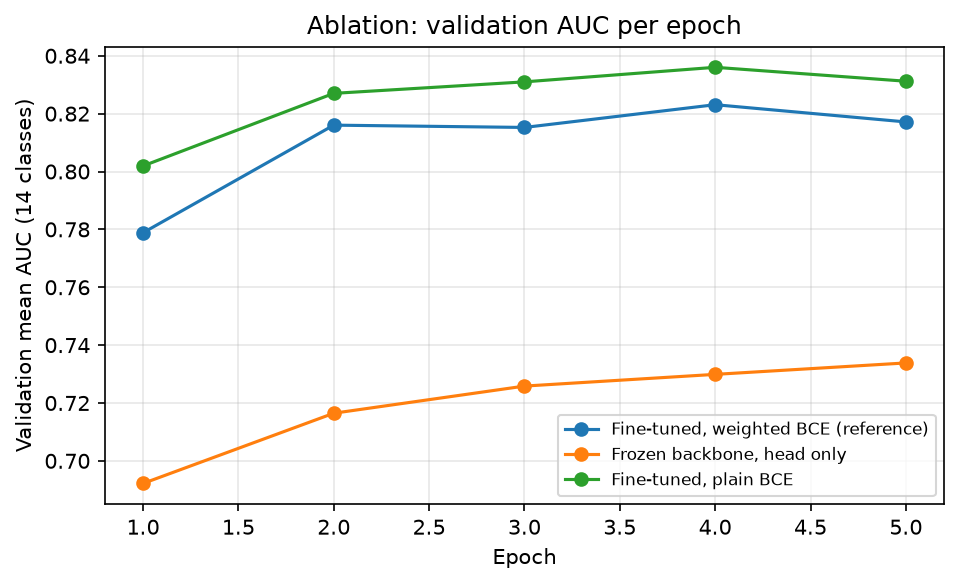
\includegraphics[width=0.75\textwidth]{ablation_curves.png}}{}
  \caption{Validation mean AUC per epoch for each ablation run.}
  \label{fig:ablation_curves}
  \end{figure}

  \paragraph{Fine-tuning matters.} Freezing the backbone and training only the final layer reaches a best validation mean AUC of 0.734, against 0.823 when the whole network is fine-tuned under the same 5-epoch budget. The frozen model is still improving at epoch 5 and both its training and validation losses fall together, so it is limited by capacity to adapt to X-rays rather than by overfitting: ImageNet features alone are not enough for this task.

\paragraph{Weighting the loss did not improve AUC.} Contrary to what we expected, plain binary cross-entropy reached 0.836 against 0.823 for the weighted loss. The plain loss is ahead at every epoch from the second on (by 0.011 to 0.016), and in 13 of the 14 classes at the best epoch, including the rare ones (Hernia $+0.009$, Pneumonia $+0.013$). So in our setup the class weights did not help the ranking quality that AUC measures. We ran a single seed per setting, so a difference of about 0.013 is suggestive and not conclusive, but its consistency across epochs and classes makes a pure fluke unlikely. The weights do change the output scale: the final model's scores are strongly over-confident (mean predicted score 0.38 against a label prevalence of 0.076, Section~\ref{sec:calibration}), which is a plausible side effect of up-weighting positives by factors up to 653. A plain-loss model with a decision threshold chosen on validation is therefore a simpler and, here, better choice. The main model (15 epochs, weighted loss, validation 0.831) was not retrained with plain BCE, and we did not evaluate the plain-loss run on the test set, so we cannot say how much test AUC this would gain.

\paragraph{Overfitting.} In the reference run the validation loss is lowest at epoch 2 (0.977) and then rises to 1.059 at epoch 5 while the training loss keeps falling (1.017 to 0.877); validation AUC peaks at epoch 4 and drops at epoch 5. This is overfitting beginning after three to four epochs. Selecting the best checkpoint by validation AUC, as we do, limits its effect, but it shows that longer training of the main model is not guaranteed to help.

\paragraph{Not run.} A strong-augmentation variant was configured but dropped to save GPU quota, so we make no claim about augmentation. All runs use the same patient-wise split; differences are measured on validation and not on the test set.

}{%
  The planned ablation study (frozen backbone versus fine-tuning, weighted versus plain binary cross-entropy, and the effect of data augmentation) was configured and is reproducible from the repository, but its results were not available when this report was written, so we draw no conclusions about these design choices here.
}


\subsection{Qualitative analysis with Grad-CAM}
Figure~\ref{fig:gradcam} shows heatmaps for two correctly detected test images. For Cardiomegaly the activation is concentrated on the cardiac silhouette; for Effusion it covers the lower lung zone, where fluid collects. This agrees with where a radiologist would look.

\begin{figure}[htbp]
\centering
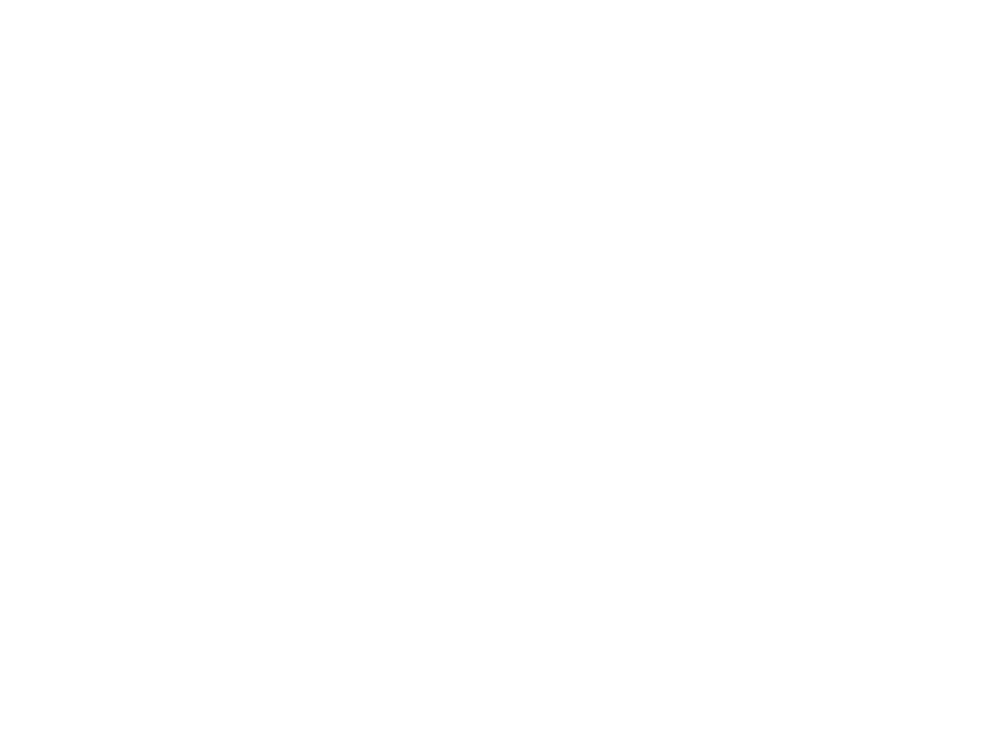
\includegraphics[width=0.9\textwidth]{gradcam_Cardiomegaly.png}\\[0.5em]
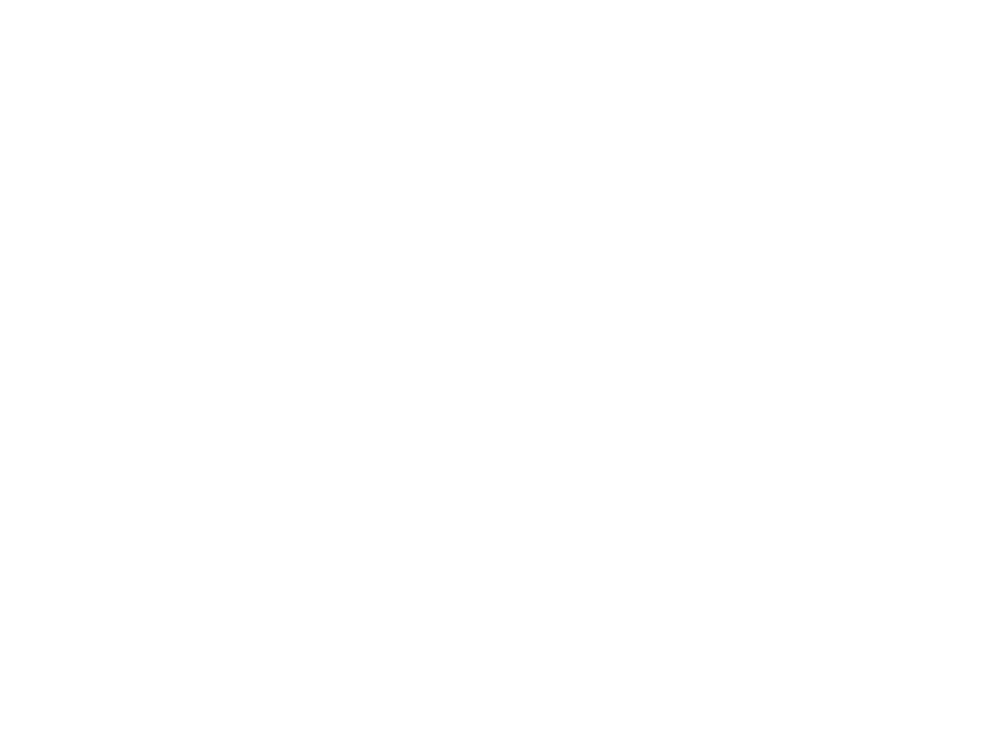
\includegraphics[width=0.9\textwidth]{gradcam_Effusion.png}
\caption{Original X-ray (left) and Grad-CAM overlay for the labelled disease (right), with the model probability. Both images belong to the official test split.}
\label{fig:gradcam}
\end{figure}

These examples are \emph{confident} cases chosen for demonstration (probabilities close to 1), not typical ones. Section~\ref{sec:localisation} measures how often the heatmaps actually point at the lesion, on 984 boxes drawn by radiologists: for DenseNet121 (trained with the benchmark recipe; this exact checkpoint was not scored) the answer is only modestly better than always pointing at the image centre, so single examples like these should not be read as evidence of correct reasoning.

% Architecture benchmark: the ablation study repeated on four architectures.
% Every number here comes from results/*.csv and the generated tables
% (scripts/analyze_models.py, scripts/collect_benchmark.py).

\section{Architecture benchmark}
\label{sec:benchmark}

\subsection{Setup}
The ablations of Section~\ref{sec:ablations} were run on DenseNet121 only, so they could not tell whether their conclusions belong to that network or to the task. We therefore repeated the same study on four ImageNet-pretrained architectures from \texttt{torchvision} that span a wide range of size and design:
DenseNet121~\cite{huang2017densenet} (7.0M parameters), ResNet50~\cite{he2016resnet} (23.5M), EfficientNet-B0~\cite{tan2019efficientnet} (4.0M) and ConvNeXt-Tiny~\cite{liu2022convnext} (27.8M).
For each one we trained three variants: fine-tuned with plain BCE, fine-tuned with the weighted BCE of Section~\ref{sec:ablations}, and a frozen backbone where only the new 14-way head is trained. DenseNet121 was trained with two extra seeds for both fine-tuned variants, giving \textbf{16 training runs}.

Everything else is identical across runs: the patient-wise split, $224\times224$ inputs with a random horizontal flip, Adam with learning rate $10^{-4}$, batch size 32, 5 epochs, mixed precision, seed 0 unless stated, and the checkpoint with the best validation mean AUC. Each run then predicts the validation and test sets and scores its Grad-CAM heatmaps (Section~\ref{sec:localisation}) in the same Kaggle job, so no number is copied between scripts by hand.

\paragraph{Making 16 runs affordable.} Decoding the 1024-pixel PNGs, not the GPU, was the bottleneck (30--45 minutes per epoch). Each job now decodes every image once into a $224\times224$ 8-bit cache (about 19 minutes for 112{,}120 images, 5.6\,GB), after which an epoch takes about 8 minutes. The cache stores exactly the output of the resize used by the transforms, so training sees the same tensors; the DenseNet121 plain-BCE run reproduces the earlier ablation (validation 0.833 against 0.836, within the seed-to-seed spread measured below).

\paragraph{Statistics.} Test AUCs come with a 95\% confidence interval from a bootstrap that resamples \emph{patients} (1{,}000 resamples), because images of one patient are not independent. Two models are compared with a \emph{paired} bootstrap on the same resamples, which gives an interval and a p-value for their difference; with 1{,}000 resamples the smallest p-value it can resolve is 0.002. This captures the uncertainty due to the finite test set, not the randomness of training; the extra DenseNet121 seeds measure the latter.

\subsection{The same study on every architecture}
\begin{figure}[ht]
\centering
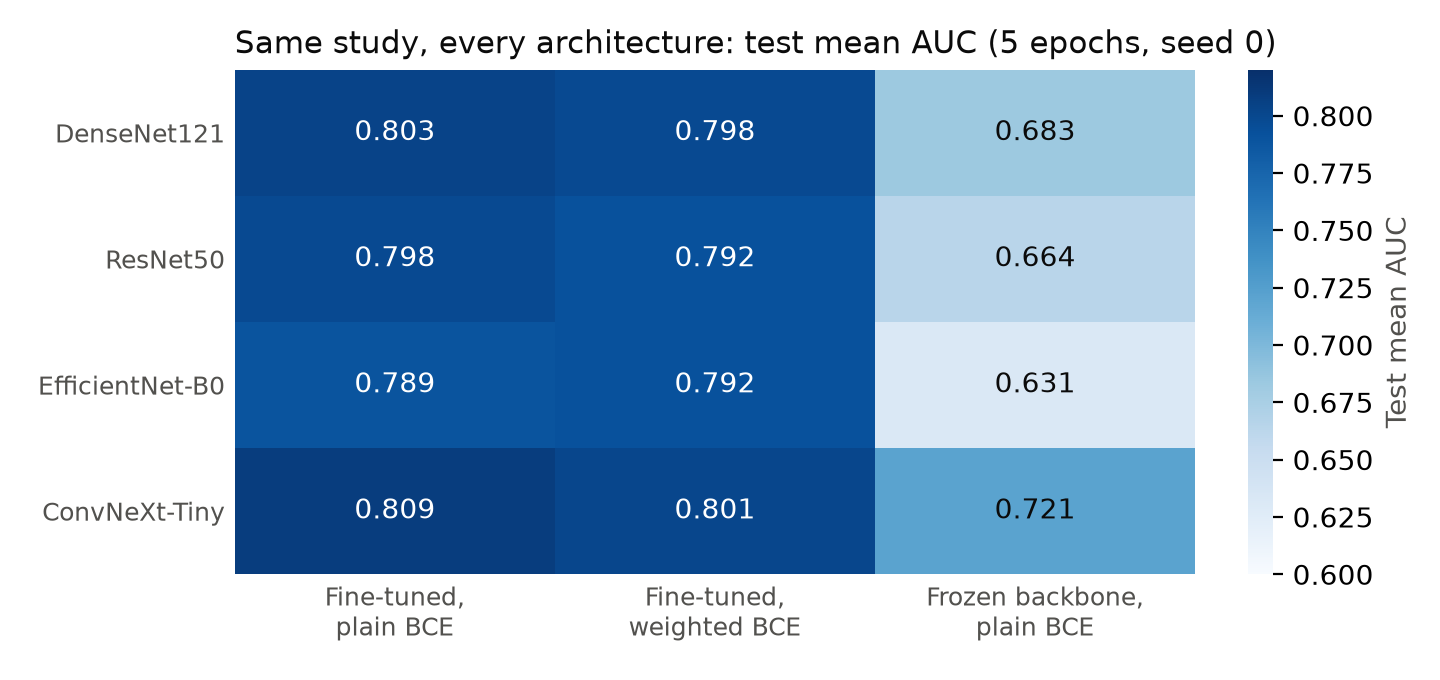
\includegraphics[width=0.82\textwidth]{grid_heatmap.png}
\caption{Test mean AUC for every architecture and variant (seed 0). The full table with confidence intervals is Table~\ref{tab:grid}.}
\label{fig:grid}
\end{figure}

\begin{table}[ht]
\centering\small
\resizebox{\textwidth}{!}{\begin{tabular}{lccc}
\toprule
Architecture & Fine-tuned, plain BCE & Fine-tuned, weighted BCE & Frozen backbone, plain BCE \\
\midrule
DenseNet121 & 0.803 [0.796, 0.808] & 0.798 [0.791, 0.803] & 0.683 [0.675, 0.691] \\
ResNet50 & 0.798 [0.791, 0.804] & 0.792 [0.785, 0.798] & 0.664 [0.655, 0.672] \\
EfficientNet-B0 & 0.789 [0.782, 0.795] & 0.792 [0.785, 0.798] & 0.631 [0.623, 0.639] \\
ConvNeXt-Tiny & \textbf{0.809 [0.802, 0.814]} & \textbf{0.801 [0.793, 0.808]} & \textbf{0.721 [0.713, 0.728]} \\
\bottomrule
\end{tabular}
}
\caption{Test mean AUC [95\% patient-bootstrap CI], official test split (25{,}596 images). Bold: best architecture in each column.}
\label{tab:grid}
\end{table}

Figure~\ref{fig:grid} and Table~\ref{tab:grid} answer the question the DenseNet ablations left open.

\paragraph{Fine-tuning matters for every architecture.} Freezing the backbone costs between 0.088 (ConvNeXt-Tiny) and 0.158 (EfficientNet-B0) of test AUC. ImageNet features are not enough for chest X-rays, whatever the network.

\paragraph{Class weighting does not help, on three architectures out of four.} The weighted loss lowers test AUC for DenseNet121 ($-0.005$, 95\% CI $[-0.009,-0.001]$, $p=0.008$), ResNet50 ($-0.006$, $[-0.010,-0.002]$, $p=0.008$) and ConvNeXt-Tiny ($-0.008$, $[-0.012,-0.004]$, $p<0.002$). EfficientNet-B0 is the exception: weighted is $0.003$ higher, but the difference is not significant ($[-0.001, 0.008]$, $p=0.11$).

\begin{table}[ht]
\centering\small
\begin{tabular}{lccc}
\toprule
DenseNet121 & Seeds & Val AUC (mean $\pm$ sd) & Test AUC (mean $\pm$ sd) \\
\midrule
Fine-tuned, plain BCE & 3 & 0.8331 $\pm$ 0.0020 & 0.8056 $\pm$ 0.0024 \\
Fine-tuned, weighted BCE & 3 & 0.8190 $\pm$ 0.0013 & 0.7968 $\pm$ 0.0009 \\
\bottomrule
\end{tabular}

\caption{DenseNet121 trained three times with different seeds per loss.}
\label{tab:seeds}
\end{table}

\paragraph{The effect is larger than the seed-to-seed noise.} The first report called the 0.013 validation gap ``suggestive only'' because it came from one run per setting. With three seeds each (Table~\ref{tab:seeds}), every plain-BCE run (test 0.803, 0.807, 0.807) is above every weighted run (0.798, 0.796, 0.796). The mean gap, 0.009 on test, is about four times the standard deviation between seeds (0.002), so it is not a lucky seed.

\subsection{Which architecture, and at what cost}
\begin{figure}[ht]
\centering
\begin{minipage}{0.49\textwidth}\centering
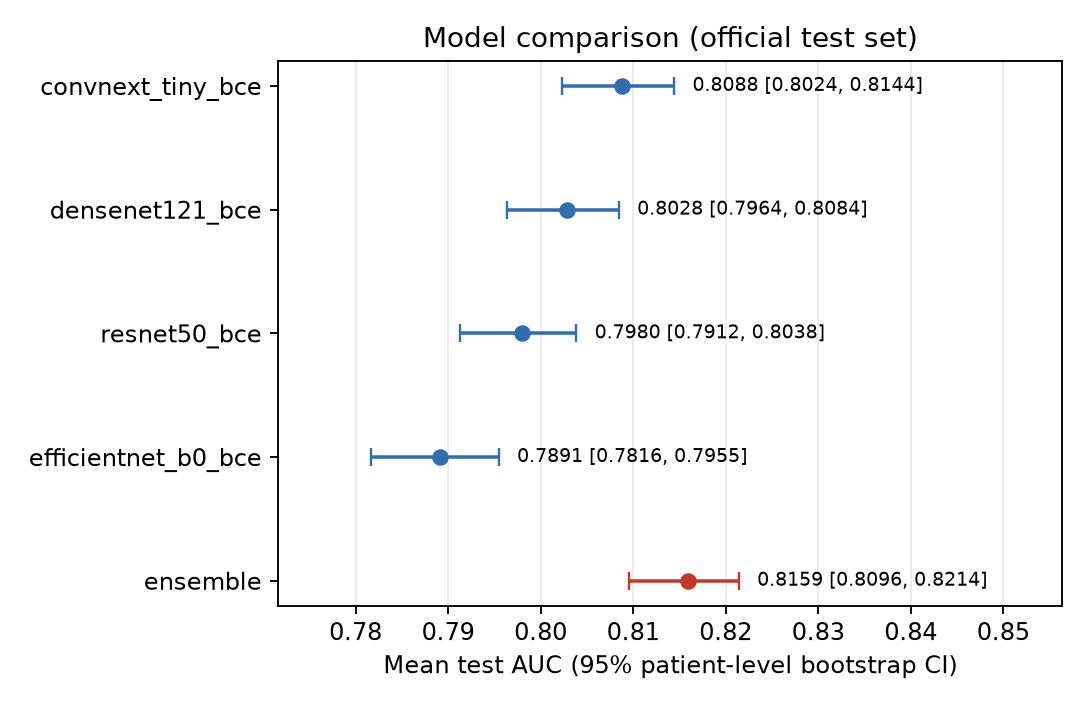
\includegraphics[width=\textwidth]{forest_auc.png}
\end{minipage}\hfill
\begin{minipage}{0.49\textwidth}\centering
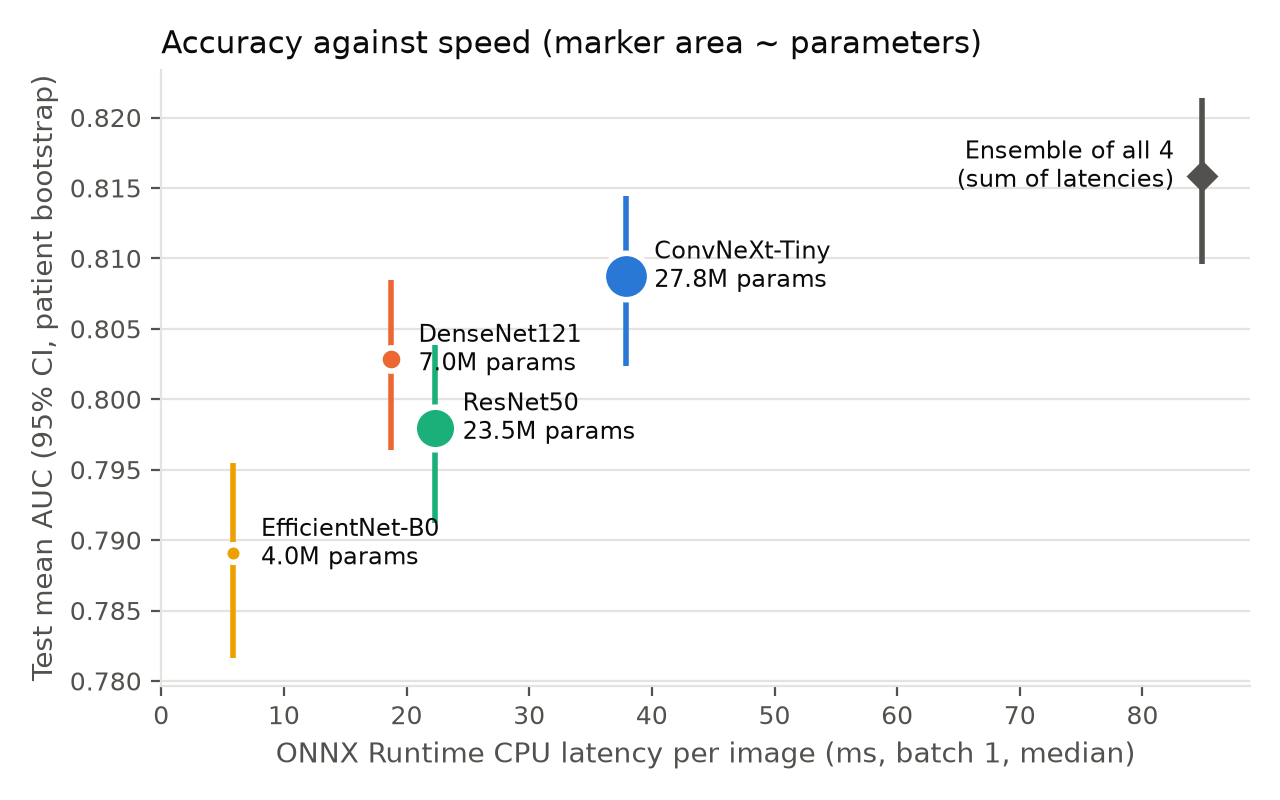
\includegraphics[width=\textwidth]{pareto.png}
\end{minipage}
\caption{Left: test mean AUC with 95\% CI for the plain-BCE models and their ensemble. Right: AUC against ONNX Runtime CPU latency per image (batch 1, median of 100 runs on a 16-thread laptop CPU); marker area is proportional to the number of parameters.}
\label{fig:forest}
\end{figure}

With the recipe fixed, ConvNeXt-Tiny is the most accurate single model (0.809 [0.802, 0.814]), followed by DenseNet121 (0.803), ResNet50 (0.798) and EfficientNet-B0 (0.789) (Figure~\ref{fig:forest}). The paired tests separate every pair (no bootstrap resample reverses any of the orders, $p<0.002$), but this needs care: ConvNeXt-Tiny is ahead of DenseNet121 by 0.006, and DenseNet121's own seeds range from 0.803 to 0.807. We did not train ConvNeXt-Tiny with several seeds, so its lead over DenseNet121 is likely but not established. Its lead over EfficientNet-B0 (0.020) is far outside that noise.

\paragraph{Ensemble.} Averaging the probabilities of the four plain-BCE models gives \textbf{0.816} [0.810, 0.821], above the best single model by 0.007 ([0.005, 0.009], $p<0.002$), a gain larger than the whole seed-to-seed range of DenseNet121. It also has the lowest calibration error (Table~\ref{tab:benchmark}). The cost is running four networks: about 85\,ms per image on CPU instead of 6--38\,ms.

\paragraph{Cost.} EfficientNet-B0 is 6.5 times faster than ConvNeXt-Tiny (5.9 against 37.9\,ms) for 0.020 less AUC; DenseNet121 (18.7\,ms) is a good middle point. Accuracy did not simply follow size: ResNet50 has 3.4 times more parameters than DenseNet121 and is less accurate.

\subsection{Calibration}
\label{sec:calibration_bench}
A temperature $T$ is fitted on the validation split for each model (minimising the BCE of $\sigma(z/T)$), and the expected calibration error (ECE, 15 bins, all classes pooled) is reported on test before and after (Table~\ref{tab:benchmark}, Figure~\ref{fig:calib_bench}). Dividing by $T$ does not change the ranking, so AUC is unchanged.

\begin{figure}[ht]
\centering
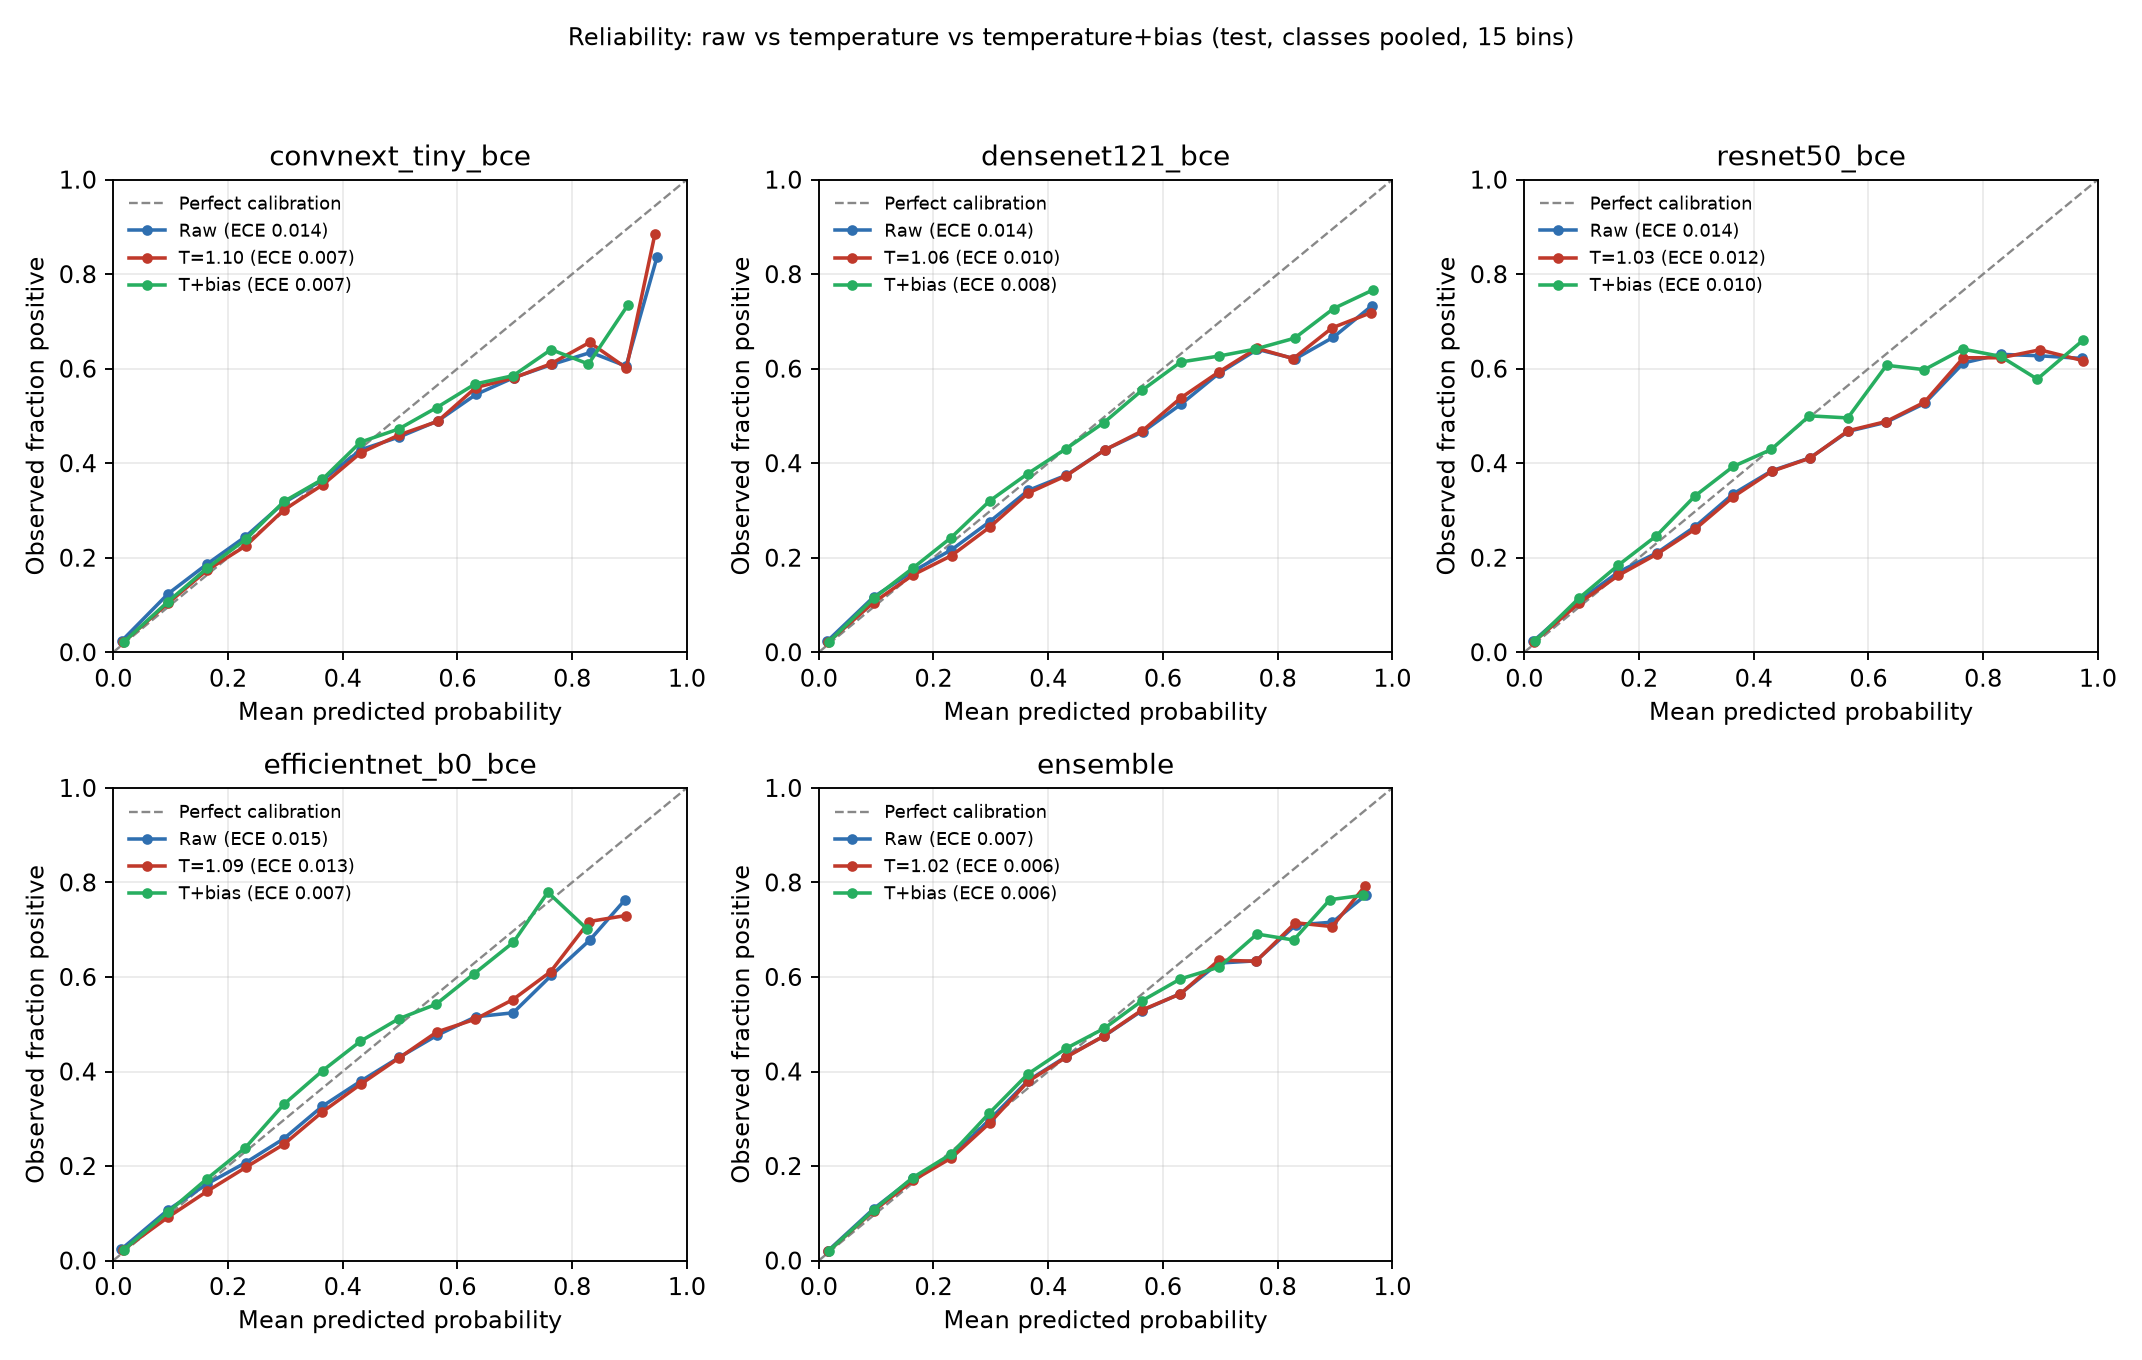
\includegraphics[width=0.95\textwidth]{calibration_before_after.png}
\caption{Reliability on the test set for the plain-BCE models: raw scores, after temperature scaling ($T$), and after temperature plus a bias term (Platt scaling), all fitted on validation.}
\label{fig:calib_bench}
\end{figure}

\paragraph{The over-confidence came from the weighted loss.} The four plain-BCE models are already close to calibrated (test ECE 0.014--0.015), and their fitted temperatures are close to 1 (1.03--1.10), lowering ECE to 0.007--0.013. Every weighted model is far off (ECE 0.33--0.36), which explains the over-confident scores of the original model (Figure~\ref{fig:calibration}). Temperature scaling cannot repair them (ECE stays at 0.33--0.36): the weights shift every logit upwards, and a scale factor cannot remove a shift. Adding a bias term (Platt scaling) does, bringing them to 0.009--0.018. The application therefore serves plain-BCE models with their temperatures, and the numbers it displays can be read as probabilities.

\subsection{Do the heatmaps point at the lesion?}
\label{sec:localisation}
The first report only showed heatmaps qualitatively. The NIH release includes 984 bounding boxes drawn by radiologists on 880 images for eight findings; none of these images is in our training split. For each box we compute the Grad-CAM heatmap of that finding (on the last convolutional block of each architecture) and measure:
\begin{itemize}
  \item the \textbf{pointing game}: whether the hottest point of the heatmap falls inside the box;
  \item the \textbf{energy}: the share of the heatmap's total mass inside the box;
  \item the \textbf{IoU} between the box and the region where the heatmap is at least half its maximum.
\end{itemize}
Two references need no model: a point placed at random lands in the box 7.8\% of the time (the mean box area), and a point always at the image centre lands in it 21.8\% of the time.

\begin{figure}[ht]
\centering
\begin{minipage}{0.49\textwidth}\centering
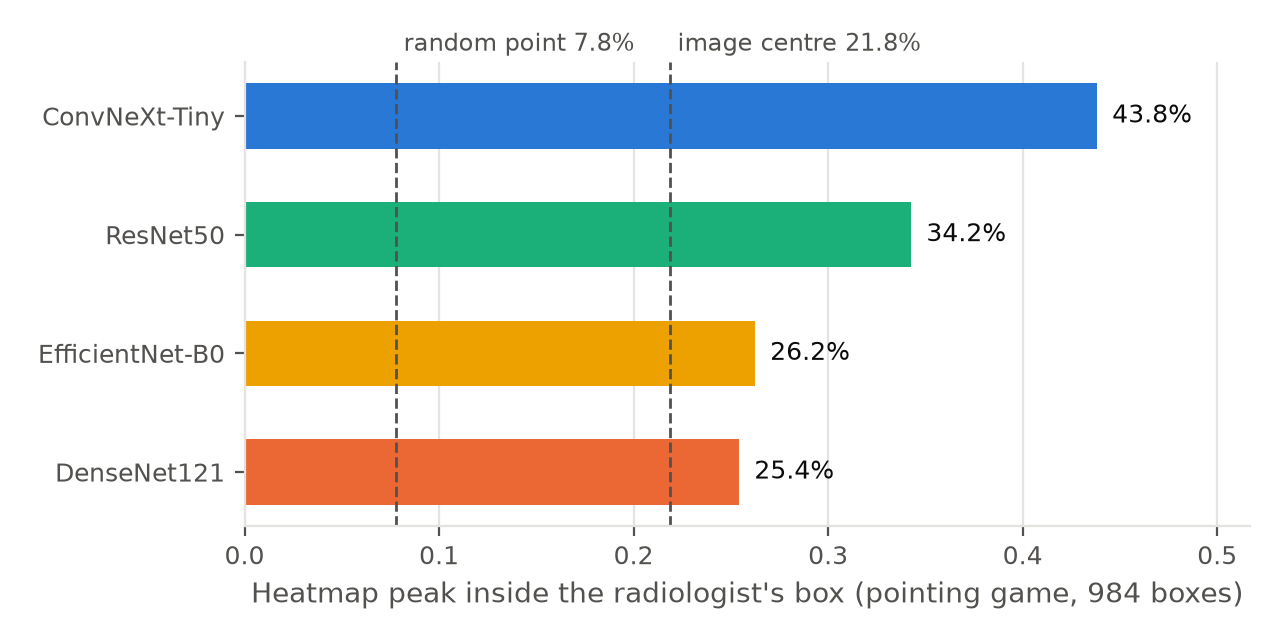
\includegraphics[width=\textwidth]{localization_bars.png}
\end{minipage}\hfill
\begin{minipage}{0.49\textwidth}\centering
\begin{tabular}{lccc}
\toprule
Model & Pointing game (hit) & Energy in box & IoU (heat $\geq$ 0.5) \\
\midrule
ConvNeXt-Tiny & 0.438 & 0.299 & 0.178 \\
ResNet50 & 0.342 & 0.227 & 0.127 \\
EfficientNet-B0 & 0.262 & 0.117 & 0.135 \\
DenseNet121 & 0.254 & 0.176 & 0.145 \\
\midrule
Random point (baseline) & 0.078 & -- & -- \\
Image centre (baseline) & 0.218 & -- & -- \\
\bottomrule
\end{tabular}

\end{minipage}
\caption{Grad-CAM localisation of the plain-BCE models against the 984 expert boxes.}
\label{fig:localisation}
\end{figure}

\begin{figure}[ht]
\centering
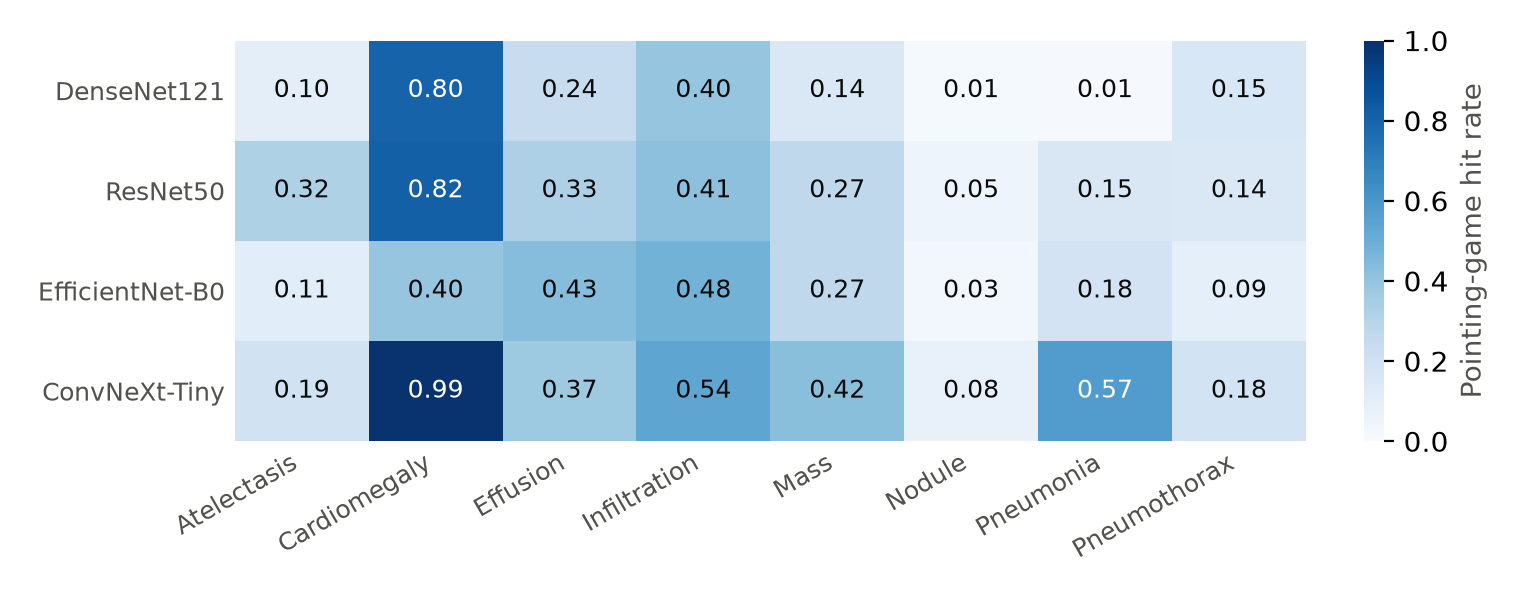
\includegraphics[width=0.85\textwidth]{localization_per_disease.png}
\caption{Pointing-game hit rate per finding. Nodule boxes cover 0.6\% of the image on average, smaller than one cell of the $7\times7$ feature map that Grad-CAM upsamples, so no model can localise them.}
\label{fig:localisation_disease}
\end{figure}

\paragraph{Results.} ConvNeXt-Tiny puts its peak inside the box for 43.8\% of the boxes, twice the centre baseline, and is also best on energy and IoU (Figure~\ref{fig:localisation}). ResNet50 follows (34.2\%). DenseNet121 (25.4\%) and EfficientNet-B0 (26.2\%) are only slightly better than always pointing at the centre. So the most accurate classifier is also the one whose explanations are most often right, but a good AUC does not by itself imply good heatmaps.

The findings differ sharply (Figure~\ref{fig:localisation_disease}). Cardiomegaly, whose box is the heart, is localised by every model except EfficientNet-B0 (ConvNeXt-Tiny 0.99). Nodules are never localised (at most 0.08), as the caption explains. For Pneumonia, ConvNeXt-Tiny points into the box 57\% of the time and DenseNet121 1\%.

\paragraph{Caveats.} These numbers are noisier than the AUCs: the three DenseNet121 plain-BCE seeds give 25.4\%, 27.0\% and 32.5\%, so only large differences such as ConvNeXt-Tiny's lead should be trusted. Two observations are consistent but unexplained: the weighted-loss models localise as well as or better than their plain counterparts (ResNet50 40.0\% against 34.2\%, EfficientNet-B0 42.6\% against 26.2\%) despite their lower AUC, and frozen backbones localise worse than the centre baseline (11.5--12.5\%). The frozen ResNet50 and EfficientNet-B0 runs have no localisation score: Grad-CAM failed on frozen backbones in those two jobs, a bug fixed before the other frozen runs, and the saved predictions were kept.

\subsection{Subgroups}
\begin{figure}[ht]
\centering
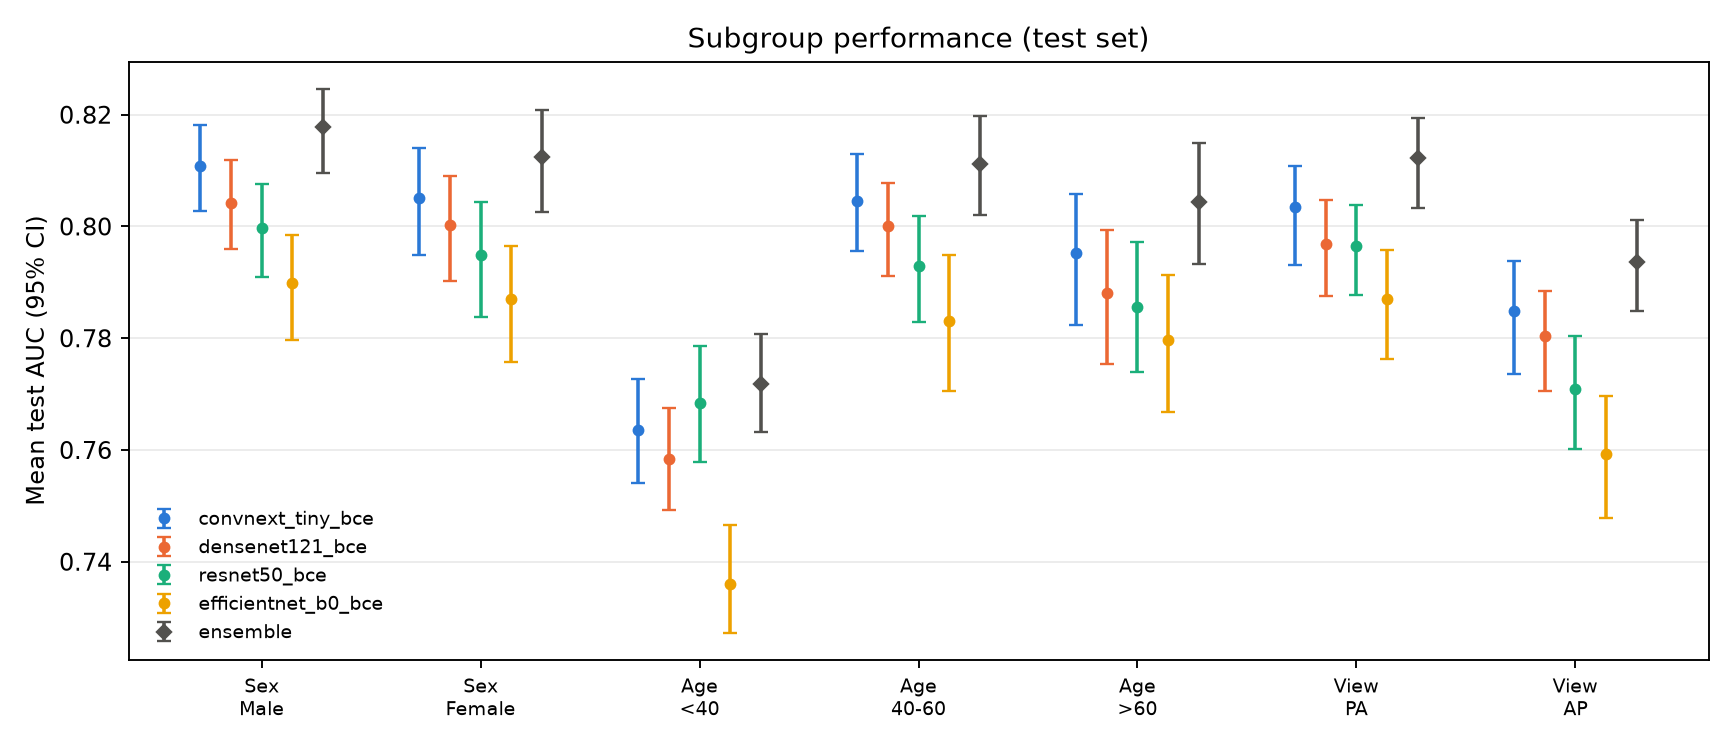
\includegraphics[width=0.95\textwidth]{subgroups.png}
\caption{Test mean AUC with 95\% CI by sex, age and view position, from the metadata of the NIH release.}
\label{fig:subgroups}
\end{figure}

\begin{table}[ht]
\centering\small
\resizebox{\textwidth}{!}{\begin{tabular}{ll rccccc}
\toprule
Group & Level & $n$ & convnext\_tiny\_bce & densenet121\_bce & resnet50\_bce & efficientnet\_b0\_bce & ensemble \\
\midrule
Sex & Male & 14,882 & 0.811 [0.803, 0.818] & 0.804 [0.796, 0.812] & 0.800 [0.791, 0.808] & 0.790 [0.780, 0.798] & 0.818 [0.810, 0.825] \\
Sex & Female & 10,714 & 0.805 [0.795, 0.814] & 0.800 [0.790, 0.809] & 0.795 [0.784, 0.804] & 0.787 [0.776, 0.797] & 0.813 [0.803, 0.821] \\
Age & <40 & 8,290 & 0.764 [0.754, 0.773] & 0.758 [0.749, 0.767] & 0.768 [0.758, 0.779] & 0.736 [0.727, 0.747] & 0.772 [0.763, 0.781] \\
Age & 40-60 & 11,733 & 0.805 [0.796, 0.813] & 0.800 [0.791, 0.808] & 0.793 [0.783, 0.802] & 0.783 [0.771, 0.795] & 0.811 [0.802, 0.820] \\
Age & >60 & 5,573 & 0.795 [0.782, 0.806] & 0.788 [0.775, 0.799] & 0.786 [0.774, 0.797] & 0.780 [0.767, 0.791] & 0.804 [0.793, 0.815] \\
View & PA & 11,096 & 0.803 [0.793, 0.811] & 0.797 [0.788, 0.805] & 0.797 [0.788, 0.804] & 0.787 [0.776, 0.796] & 0.812 [0.803, 0.819] \\
View & AP & 14,500 & 0.785 [0.774, 0.794] & 0.780 [0.771, 0.788] & 0.771 [0.760, 0.780] & 0.759 [0.748, 0.770] & 0.794 [0.785, 0.801] \\
\bottomrule
\end{tabular}
}
\caption{Subgroup test mean AUC [95\% CI]. $n$ is the number of test images in the group.}
\label{tab:subgroups}
\end{table}

All models behave the same way across subgroups (Figure~\ref{fig:subgroups}, Table~\ref{tab:subgroups}). There is no gap between men and women. Two gaps are clear and shared by every architecture:
\begin{itemize}
  \item patients under 40 are harder (ConvNeXt-Tiny 0.764 against 0.805 for 40--60);
  \item AP films are harder than PA films (0.785 against 0.803). AP films are usually taken at the bedside, on patients too ill to stand, with more overlapping devices and lower image quality.
\end{itemize}
We report these gaps but cannot separate their causes, such as different disease mixes per group and label noise, with the data available.

\subsection{Full results}
\begin{table}[ht]
\centering
\resizebox{\textwidth}{!}{\begin{tabular}{lcrrrrrrr}
\toprule
Model & Mean AUC [95\% CI] & AP & ECE & ECE (T) & $T$ & ECE (T+b) & Params & Latency (ms) \\
\midrule
convnext\_tiny\_bce & 0.8088 [0.802, 0.814] & 0.276 & 0.014 & 0.007 & 1.10 & 0.007 & 27.8M & 37.9 \\
convnext\_tiny\_frozen & 0.7208 [0.713, 0.728] & 0.156 & 0.013 & 0.012 & 1.01 & 0.012 & 27.8M & -- \\
convnext\_tiny\_weighted & 0.8011 [0.793, 0.808] & 0.267 & 0.336 & 0.339 & 1.11 & 0.009 & 27.8M & -- \\
densenet121\_bce & 0.8028 [0.796, 0.808] & 0.259 & 0.014 & 0.010 & 1.06 & 0.008 & 7.0M & 18.7 \\
densenet121\_bce\_s1 & 0.8067 [0.800, 0.812] & 0.279 & 0.016 & 0.014 & 1.06 & 0.007 & 7.0M & -- \\
densenet121\_bce\_s2 & 0.8071 [0.801, 0.812] & 0.276 & 0.009 & 0.009 & 1.00 & 0.006 & 7.0M & -- \\
densenet121\_frozen & 0.6826 [0.675, 0.691] & 0.136 & 0.011 & 0.014 & 0.96 & 0.015 & 7.0M & -- \\
densenet121\_weighted & 0.7978 [0.791, 0.803] & 0.259 & 0.359 & 0.361 & 1.07 & 0.017 & 7.0M & -- \\
densenet121\_weighted\_s1 & 0.7963 [0.789, 0.802] & 0.264 & 0.338 & 0.337 & 0.96 & 0.011 & 7.0M & -- \\
densenet121\_weighted\_s2 & 0.7963 [0.789, 0.803] & 0.255 & 0.329 & 0.330 & 1.03 & 0.016 & 7.0M & -- \\
efficientnet\_b0\_bce & 0.7891 [0.782, 0.795] & 0.247 & 0.015 & 0.013 & 1.09 & 0.007 & 4.0M & 5.9 \\
efficientnet\_b0\_frozen & 0.6310 [0.623, 0.639] & 0.118 & 0.017 & 0.017 & 0.98 & 0.018 & -- & -- \\
efficientnet\_b0\_weighted & 0.7925 [0.785, 0.798] & 0.252 & 0.339 & 0.342 & 1.11 & 0.013 & 4.0M & -- \\
resnet50\_bce & 0.7980 [0.791, 0.804] & 0.252 & 0.014 & 0.012 & 1.03 & 0.010 & 23.5M & 22.3 \\
resnet50\_frozen & 0.6640 [0.655, 0.672] & 0.127 & 0.015 & 0.017 & 0.98 & 0.017 & -- & -- \\
resnet50\_weighted & 0.7920 [0.785, 0.798] & 0.256 & 0.329 & 0.333 & 1.15 & 0.011 & 23.5M & -- \\
\midrule
ensemble & \textbf{0.8159} [0.810, 0.821] & 0.283 & 0.007 & 0.006 & 1.02 & 0.006 & -- & -- \\
\bottomrule
\end{tabular}
}
\caption{All 16 runs and the ensemble on the test set: mean AUC [95\% CI], average precision, ECE raw / after temperature scaling / after temperature and bias, the fitted temperature, parameters and CPU latency (measured for the served models). Run names are \texttt{architecture\_variant[\_seed]}.}
\label{tab:benchmark}
\end{table}


\section{System}
The models are delivered as a small web application (Figure~\ref{fig:arch}).

\begin{figure}[htbp]
\centering
\small
\begin{tabular}{@{}c@{\ \ }c@{\ \ }c@{\ \ }c@{\ \ }c@{}}
Browser (React) & $\rightarrow$ & nginx & $\rightarrow$ & FastAPI (ONNX Runtime; PyTorch for Grad-CAM)
\end{tabular}
\caption{Architecture. nginx serves the single-page app and proxies \texttt{/api} to the backend, so the browser makes no cross-origin calls.}
\label{fig:arch}
\end{figure}

\paragraph{Backend.} The trained PyTorch model is exported to ONNX. An automatic check confirms the exported model matches PyTorch (largest output difference about $1.4\times10^{-6}$), and the API's probabilities match PyTorch to about $1.5\times10^{-7}$. Preprocessing in the API is implemented in NumPy and tested to be identical to the training-time transforms. The endpoints are:
\begin{itemize}
  \item \texttt{GET /health} and \texttt{GET /model/metadata} (classes, input size, validation and test AUC, model hash);
  \item \texttt{GET /models}: the served models with their test AUC, temperature and size, plus the ensemble;
  \item \texttt{POST /predict?model=\dots}: all 14 probabilities, the top five, and latency, for one model or the ensemble;
  \item \texttt{POST /predict/visualize}: the same plus a Grad-CAM overlay. Grad-CAM needs gradients, which ONNX Runtime does not provide, so this endpoint loads the PyTorch checkpoint lazily;
  \item \texttt{POST /predict/compare}: every model and the ensemble on the same image, each with its heatmap for a chosen disease.
\end{itemize}
The served models are listed in \texttt{models/registry.json}, generated from the benchmark results: architecture, file paths, validation and test AUC, and the temperature fitted on validation. Probabilities are computed as $\sigma(z/T)$ with that temperature, and the ensemble averages the members' probabilities (and heatmaps). All four architectures pass the same ONNX parity check against PyTorch (largest relative output difference $1.7\times10^{-5}$).
Uploads are decoded for real, not trusted by file type: non-images are rejected with a 400 and files over 10~MB with a 413. Cross-origin access is limited to configured origins.

\paragraph{Frontend.} A React and TypeScript single-page app supports drag-and-drop upload, an example gallery of eight test-set X-rays, webcam capture (implemented, but not yet tested with a physical camera), probability bars, a Grad-CAM overlay selectable per disease, and a display of model metadata and latency. Stale responses are discarded so a slow heatmap cannot overwrite a newer upload. A model selector switches between the four models and the ensemble, and a comparison view runs all of them on the same image (Figure~\ref{fig:app_compare}). Agreement between architectures is more convincing than one model alone; disagreement, such as a heatmap that points elsewhere, is a reason for caution.

\begin{figure}[htbp]
\centering
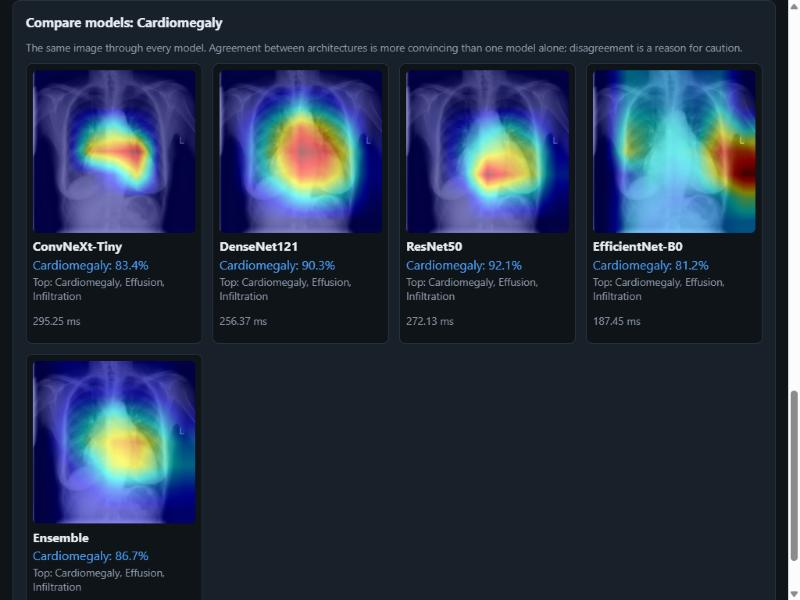
\includegraphics[width=0.85\textwidth]{app_compare.jpg}
\caption{Comparison view of the application, running in Docker, on a test-set X-ray labelled Cardiomegaly. All models give a high calibrated probability; three heatmaps cover the heart, while EfficientNet-B0's points at the edge of the left lung, consistent with its low Cardiomegaly localisation score (Figure~\ref{fig:localisation_disease}).}
\label{fig:app_compare}
\end{figure}

\paragraph{Performance.} On a laptop CPU, \texttt{/predict} takes about 25~ms per image. A Grad-CAM heatmap takes about 0.3~s once warm, but the first one after the server starts takes 7 to 13~s because PyTorch and the model are loaded; the interface shows a loading state for this.

\paragraph{Engineering.} Model weights are versioned with DVC and stored on a DagsHub remote; git holds only a small pointer file. Training is configured by YAML files and tracked with MLflow. Automated tests (data splitting, model shapes, ONNX parity, the API with a stub model, and an end-to-end training smoke test on synthetic data) run in GitHub Actions together with linting, the frontend build and the Docker image build. The application is started with \texttt{docker compose up}; weights are mounted into the container and never baked into an image.

\subsection{The role of Docker}
\label{sec:docker}
Docker is used to \emph{deliver} the trained models, not to train them: training needs a GPU and runs as Kaggle jobs, and its environment is pinned by the job scripts and the configuration files. What Docker solves is everything after training (Figure~\ref{fig:docker}).

\begin{figure}[ht]
\centering\small
\setlength{\tabcolsep}{4pt}
\begin{tabular}{c c c c c}
\fbox{\begin{minipage}{0.17\textwidth}\centering Browser\\[-0.2em]{\footnotesize React app}\end{minipage}}
& $\xrightarrow{\ \texttt{:8080}\ }$ &
\fbox{\begin{minipage}{0.24\textwidth}\centering \textbf{web} container\\[-0.2em]{\footnotesize nginx: static app, proxies \texttt{/api}}\\[-0.2em]{\footnotesize image 76\,MB}\end{minipage}}
& $\xrightarrow{\ \texttt{/api}\ }$ &
\fbox{\begin{minipage}{0.30\textwidth}\centering \textbf{api} container\\[-0.2em]{\footnotesize FastAPI, ONNX Runtime, PyTorch (Grad-CAM)}\\[-0.2em]{\footnotesize image 2.65\,GB, health-checked}\end{minipage}}\\[0.6em]
& & & & $\uparrow$ {\footnotesize read-only volume}\\[0.2em]
& & & &
\fbox{\begin{minipage}{0.30\textwidth}\centering \texttt{./models} on the host\\[-0.2em]{\footnotesize \texttt{registry.json}, 4 ONNX + 4 PyTorch models (DVC)}\end{minipage}}
\end{tabular}
\caption{Deployment with Docker Compose. One command, \texttt{docker compose up}, builds and starts both containers.}
\label{fig:docker}
\end{figure}

\begin{itemize}
  \item \textbf{Reproducible environment.} The API depends on specific versions of Python, PyTorch, ONNX Runtime and the Grad-CAM library. The image freezes them, so the service behaves the same on our laptops, a grader's machine or a server, without installing anything but Docker. Before Docker, running the demo meant reproducing a Python environment with several gigabytes of packages by hand.
  \item \textbf{Separation of concerns.} The frontend is built once into static files and served by nginx in its own small image; the model server is a separate container. nginx also proxies \texttt{/api} to the backend, so the browser talks to a single origin and needs no cross-origin exceptions. Each part can be rebuilt, restarted or scaled without touching the other.
  \item \textbf{Code and weights are separate.} The image contains code and libraries only. The model files are mounted read-only from \texttt{./models}, where DVC places them. Changing or adding a model means editing \texttt{models/registry.json} and restarting, with no image rebuild; this is how the four benchmark models were added to the app.
  \item \textbf{Operations.} The API image declares a health check on \texttt{/health}, so Docker reports whether the model server is actually answering; Compose restarts either container if it stops, and starts the web container after the API.
  \item \textbf{Checked continuously.} GitHub Actions builds both images (\texttt{docker compose build}) on every change, so a broken Dockerfile is caught before it reaches anyone.
\end{itemize}
We verified the stack end to end with the four benchmark models: \texttt{/api/health} answers through nginx, \texttt{/api/models} lists the four models and the ensemble, and the comparison view below runs inside the containers.


\section{Limitations and ethics}
\begin{itemize}
  \item \textbf{Not a medical device.} The system is a research and educational demo. It must not be used for diagnosis, and the interface says so.
  \item \textbf{Label noise.} Labels are machine-extracted from reports, so reported AUCs measure agreement with noisy labels, not with a radiologist's ground truth.
  \item \textbf{Single dataset, single hospital.} We did no external validation, so performance on other populations and scanners is unknown.
  \item \textbf{Training randomness measured for one architecture only.} Confidence intervals cover the finite test set; seed-to-seed variation was measured for DenseNet121 only (standard deviation 0.002 of test AUC). ConvNeXt-Tiny's 0.006 lead over DenseNet121 is therefore likely but not established.
  \item \textbf{Short training.} Benchmark runs use 5 epochs, the budget of the original ablations; longer schedules could change the ranking, particularly for the larger networks.
  \item \textbf{Low resolution.} Images are reduced to $224\times224$, which can hide small findings: no model localises nodules (Section~\ref{sec:localisation}).
  \item \textbf{Calibration is global, precision is low.} One temperature per model makes the scores calibrated when pooled over all classes, but individual rare classes can still be off. At a useful sensitivity the precision remains low (mean 0.14 for the first model), because most findings are rare.
  \item \textbf{Localisation is noisy and partial.} Grad-CAM scores vary between seeds (DenseNet121: 25--33\%), only eight findings have boxes, and two frozen runs were not scored.
  \item \textbf{Horizontal flip.} Flipping moves the heart to the wrong side of the image, which may matter for findings such as Cardiomegaly.
\end{itemize}

\section{Conclusion}
We built an end-to-end system: a leakage-free training pipeline, visual explanations, and a tested, containerised application. Repeating the ablation study on four architectures turned single-run observations into findings:
\begin{itemize}
  \item fine-tuning is essential for every network;
  \item class weighting does not improve AUC and is what made the first model over-confident;
  \item plain cross-entropy with temperature scaling gives calibrated probabilities.
\end{itemize}
ConvNeXt-Tiny is the strongest single model (test AUC 0.809) and also the one whose heatmaps most often point at the lesion; averaging four architectures reaches 0.816. Measuring the explanations showed that a good AUC does not guarantee good heatmaps, which is why the application lets the user compare models side by side. Natural next steps are seeds for every architecture, higher input resolution, longer training, label-noise-aware training and external validation on another hospital's data.

\begin{thebibliography}{9}
\bibitem{wang2017chestxray} X.~Wang, Y.~Peng, L.~Lu, Z.~Lu, M.~Bagheri, R.~Summers. ChestX-ray8: Hospital-scale chest X-ray database and benchmarks on weakly-supervised classification and localization of common thorax diseases. \emph{CVPR}, 2017.
\bibitem{huang2017densenet} G.~Huang, Z.~Liu, L.~van~der~Maaten, K.~Weinberger. Densely connected convolutional networks. \emph{CVPR}, 2017.
\bibitem{selvaraju2017gradcam} R.~Selvaraju, M.~Cogswell, A.~Das, R.~Vedantam, D.~Parikh, D.~Batra. Grad-CAM: Visual explanations from deep networks via gradient-based localization. \emph{ICCV}, 2017.
\bibitem{he2016resnet} K.~He, X.~Zhang, S.~Ren, J.~Sun. Deep residual learning for image recognition. \emph{CVPR}, 2016.
\bibitem{tan2019efficientnet} M.~Tan, Q.~Le. EfficientNet: Rethinking model scaling for convolutional neural networks. \emph{ICML}, 2019.
\bibitem{liu2022convnext} Z.~Liu, H.~Mao, C.-Y.~Wu, C.~Feichtenhofer, T.~Darrell, S.~Xie. A ConvNet for the 2020s. \emph{CVPR}, 2022.
\end{thebibliography}

\end{document}
